%%%%%%%%%%%%%%%%%%%%%%%%%%%%%%%%%%%%%%%%%
% Beamer Presentation
% LaTeX Template
% Version 1.0 (10/11/12)
%
% This template has been downloaded from:
% http://www.LaTeXTemplates.com
%
% License:
% CC BY-NC-SA 3.0 (http://creativecommons.org/licenses/by-nc-sa/3.0/)
%
%%%%%%%%%%%%%%%%%%%%%%%%%%%%%%%%%%%%%%%%%

%----------------------------------------------------------------------------------------
%	PACKAGES AND THEMES
%----------------------------------------------------------------------------------------

\documentclass{beamer}

\mode<presentation> {
\usetheme{Madrid}
\usefonttheme{serif} 
\setbeamertemplate{navigation symbols}{} % To remove the navigation symbols from the 
}
\usepackage{lmodern}  
\usepackage{graphicx} % Allows including images
\usepackage{booktabs} % Allows the use of \toprule, \midrule and \bottomrule in tables
\usepackage[T1]{fontenc}
\usepackage[utf8]{inputenc}
\usepackage{amsmath}
\usepackage{caption} 
\usepackage{color}
\usepackage[czech]{babel}
\usepackage{lmodern}  
\usepackage{rotating}
\usepackage{scrextend}
\usepackage{pifont}
\usepackage{hyperref}
\usepackage{bm}
\usepackage{tikz}
\usetikzlibrary{arrows,positioning}
\usetikzlibrary{calc}
%
\newcommand*\circled[1]{\tikz[baseline=(char.base)]{
    \node[shape=circle,draw=red,inner sep=2pt] (char) {#1};}}
%
\newcommand*\circledd[1]{\tikz[baseline=(char.base)]{
    \node[shape=circle,draw=ProcessBlue, dashed, inner sep=2pt] (char) {#1};}}
%
\newcommand{\mytikzmark}[2]{%
  \tikz[remember picture,inner sep=0pt,outer sep=0pt,baseline,anchor=base] 
    \node (#1) {\ensuremath{#2}};}
%
%
\newcommand*{\boxcolor}{Red}
\makeatletter
\renewcommand{\boxed}[1]{\textcolor{\boxcolor}{%
\tikz[baseline={([yshift=-1ex]current bounding box.center)}] \node [rectangle,semithick, minimum width=1ex,draw, dashed] {\normalcolor\m@th$\displaystyle#1$};}}
 \makeatother
%
%------------------------------
%	TITLE PAGE
\title[Block 6]{Praktikum z ekonometrie} 
\author{VŠE Praha} 
\institute[4EK417] 
{
% Your institution for the title page
\medskip
\textit{Tomáš Formánek} % Your email address
}
\date{} % Date, can be changed to a custom date
%------------------------------
\begin{document}
\begin{frame}
\titlepage % Print the title page as the first slide
\end{frame}
%------------------------------
\begin{frame}
\frametitle{Block 6 – Treatment effects – Outline
} 
\tableofcontents 
\end{frame}
%------------------------------
\section{Treatment effects: Introduction}
\begin{frame}{Treatment effects: Introduction}
\begin{itemize}
    \item \textbf{Treatment effect analysis:} to evaluate the impact of intervention (treatment) on some \textbf{outcome} of interest.
    \bigskip
    \item Response to treatment is evaluated relative to a benchmark:  \\no treatment (control) or different treatment. 
    \bigskip
    \item Analysis of treatment effect is typically based on regression models, with outcome as the dependent variable.
    \bigskip
    \item Treatment effect analysis is generally based on the framework of Rubin's causal model. 
\end{itemize}
\end{frame}
%------------------------------
\begin{frame}{Treatment effects: Introduction}
\textbf{Examples}\\ \medskip
\begin{itemize}
    \item Wage effect of enrollment in a skill-training program.
    \medskip
    \item Health effects (speed of recovery), if new drug / medical procedure is used.
    \medskip
    \item Student performance upon being educated in small classes as opposed to large classes (being in a small class is the treatment). 
\end{itemize}
\bigskip
\textbf{Key topics of the analysis:}\\
Treatment participation: random assignment or self selection?\\
Treatment effects: actual effects or influence by confounding factors?\\
\bigskip
\textbf{Multiple treatments:} If treatment varies in intensity or type. Same principle of analysis, the choice of benchmark is more flexible.
\end{frame}
%------------------------------
% Define box and box title style
\tikzstyle{mybox} = [draw=blue!35, fill=white, very thick,
    rectangle, rounded corners, inner sep=1pt, inner ysep=10pt]
\tikzstyle{fancytitle} =[fill=blue!35, text=black]
%---------------------------------
\begin{frame}{Treatment effects: Basic notation \& terminology}
\begin{itemize}
    \item Every $i$th individual in a population has a potential outcome $y_i$ and can be exposed to treatment $C_i=\{0;1\}$. 
    \medskip
    \item $y_{i1} = y_i | (C_i = 1) $ for the treated, and \\
    $y_{i0} = y_i | (C_i = 0)$ for the non-treated.
    \medskip
    \item Average treatment effect (averaged across population):
    $$\textnormal{ATE} = E \left[ y_{i1}-y_{i0}\right],$$
    and the $i$th observation only exist in one of the two states.
    \medskip
    \item \textbf{Average treatment effect of the treated} is more of interest:
    $$\textnormal{ATET} = E \left[ y_{i1}-y_{i0} | C_i = 1\right],$$
    and the second term $y_{i0}$ is a missing counterfactual. 
    \medskip
    \item Individuals will only exist in one state: treated/untreated. Multiple assumptions apply for ATE/ATET estimation.
\end{itemize}  
\end{frame}
%------------------------------
\begin{frame}{Treatment effects: Study \& data types}
\textbf{Types of studies and data used for TE analysis}:\\
\begin{itemize}
    \item Scientific experiments under randomisation: assignment into treated and control groups is random. \\ \medskip Relatively rare in socio-economic studies. 
    \bigskip
    \item Observational studies (natural experiments, quasi-experiments): assignment into treatment and control group is not random. \\ \medskip
    
    Self-selection bias: if treatment (participation) is optional, individuals who choose to participate may be systematically different from non-participants.
\end{itemize}
\end{frame}
%---------------------------------
\begin{frame}{Treatment effects: Study \& data types}
\begin{tikzpicture}
\node [mybox] (box){%
\begin{minipage}{0.50\textwidth}
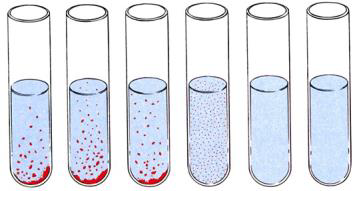
\includegraphics[width=\textwidth, height=2.89cm]{./IMG/Obrazek1}
\begin{itemize}
\scriptsize
\item Test tubes identical except for catalyst
\item Measure: Effect at different catalyst volumes (reaction speed, product volume, \dots)
\item Perform the experiment $n$-times
\item Control for other factors (heat, \dots)
\item Estimate average effects \& standard errors
\end{itemize}
\end{minipage}
};
\node[fancytitle, right=5pt,  rounded corners] at (box.north west) {\scriptsize Scientific experiment};
\end{tikzpicture}%
\begin{tikzpicture}
\node [mybox] (box){%
\begin{minipage}{0.50\textwidth}
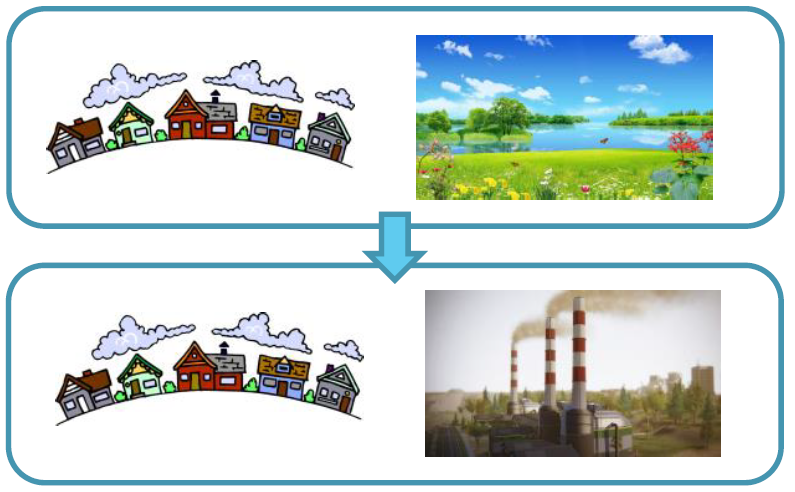
\includegraphics[width=\textwidth]{./IMG/Obrazek2}
\begin{itemize}
\scriptsize
\item Garbage incinerator is built in one given
suburban area over time
\item How do we estimate the effect on
individual house-prices?
\item Identical control group does not exist…
\item Different estimators exist -- multiple
assumptions apply!
\end{itemize}
\end{minipage}
};
\node[fancytitle, right=5pt,  rounded corners] at (box.north west) {\scriptsize Natural experiment (quasi-experiment)};
\end{tikzpicture}%
\end{frame}
%---------------------------------





%---------------------------------
\begin{frame}{Treatment effects: Introduction}
\small
For evaluation of scientific experiments (if treatment/intervention is exogenous), one can formulate a regression model with a treatment-related dummy variable, as follows:
$$
y_i = \bm{x}_i^{\prime}\bm{\beta} + \delta D_i + \varepsilon_i,
$$
where $D_i = 1$ if the $i$th individual (CS unit) is in the treatment group and zero otherwise (for the control group). \\
\medskip
For a simplified scenario, we can leave out covariates $\bm{x}$ and compare two groups (treated/untreated):
$$
y_i = \beta_0 + \delta D_i + \varepsilon_i,
$$    
with $\hat{\beta}_0 = [\overline{y}|_{D_i=0}]$ being the average outcome for the untreated,\\
and $\hat{\delta} = [\overline{y}|_{D_i=1}] - [\overline{y}|_{D_i=0}]$ as the mean difference between the two groups.\\
\bigskip
\textbf{Note:} exogeneity of $D$ is crucial for estimation of the treatment effect. Inclusion of $\bm{x}_i^{\prime}\bm{\beta}$ in the equation doesn't change the general interpretation of $\delta$.
\end{frame}
%---------------------------------
\section{Treatment effects analysis - exogenous assignment \& DiD estimator}
\begin{frame}{DiD estimator: Policy analysis with pooled CS data} 
\small
DiD refers to a popular approach towards policy analysis \& evaluation, based on models with two dummy variables: $T$ differentiates between two time periods (before/after treatment) and $D$ distinguishes the two groups (treatment/control). \\ \medskip 
DiD estimator is based on model: \\ 
$$y_{it}=\beta_0 + \beta_1 D_i + \beta_2 T_t + \delta_1 (D_i T_t) + \varepsilon_{it},$$
where:
\begin{itemize}
\item $i=1, \dots, N;~~t=1,2$. \\
\item[$T_t$] is a time dummy, $T_1=0$ is the first (pre-treatment) period and \\$T_2 = 1$ is the second period (post treatment),
\item[$D_i$] is a treatment dummy, $D_i=1$ for the treated,
\item[$D_i T_t$] is an interaction element, i.e. $(D_i\! \cdot \! T_t)$,
\item[$\delta_1$] is the DiD estimator (coefficient),
\item adding $\bm{x}_{it}^{\prime}\bm{\beta}$ to model doesn't change the general interpretation of $\delta_1$.
\end{itemize}
\end{frame}
%---------------------------------
\begin{frame}{DiD estimator: Policy analysis with pooled CS data}
\vfill
{\footnotesize \underline{\textbf{DiD estimator example: In-house employee training for women}} \\
\underline{\textbf{returning from maternal leave \& its wage effect}}} \\
\medskip
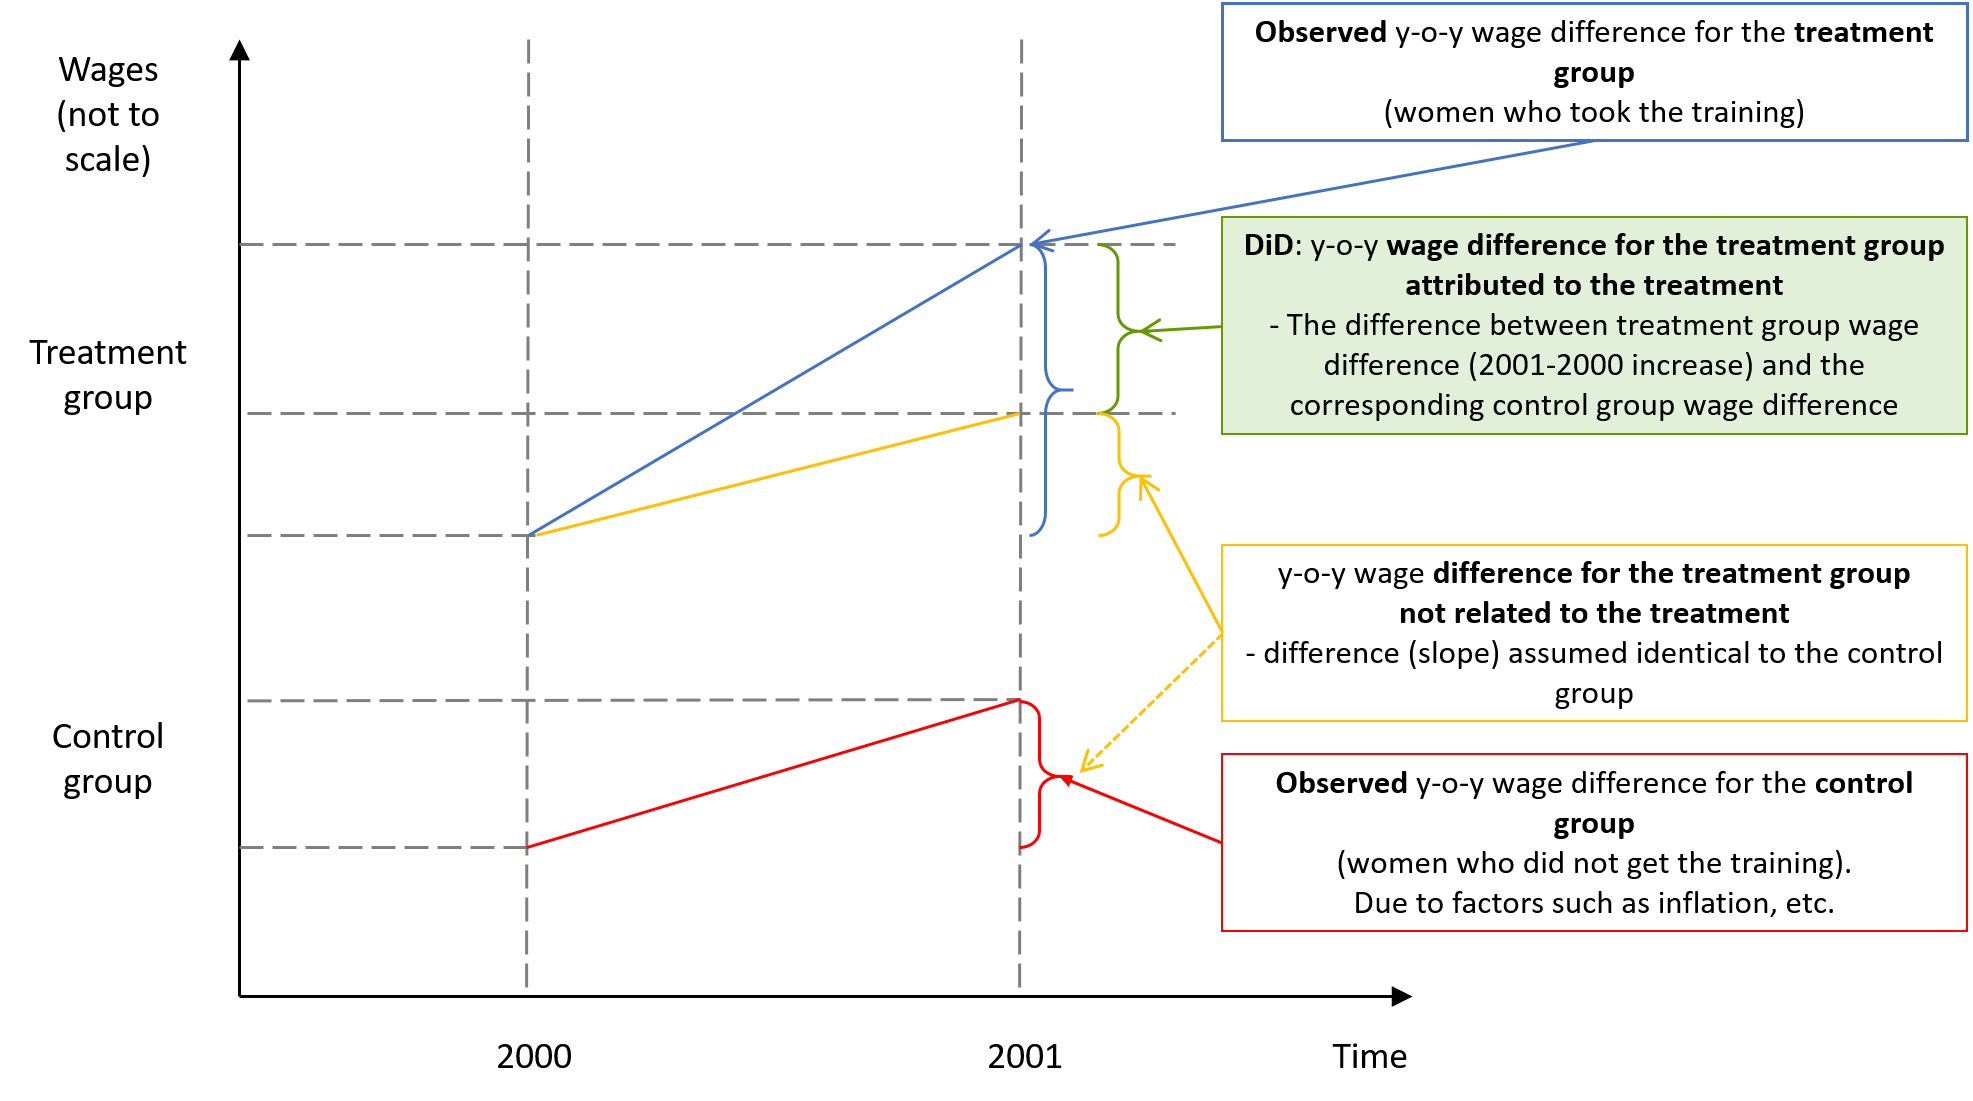
\includegraphics[width=\textwidth]{./IMG/Obrazek3}
\end{frame}
%---------------------------------
\begin{frame}{DiD estimator: Policy analysis with pooled CS data}
\small 
\underline{\textbf{DiD estimator:}} we use LRMs to compare changes in conditional means for the treatment and control groups.
\begin{itemize}
\item Group specific (treatment/control) and time specific effects are addressed.
\end{itemize}
\medskip
\underline{\textbf{Assumptions:}}
\begin{itemize}
\item Exogeneity of treatment (of the $D_i$ variable): unbiased DiD estimates require that the treatment (individual being subject to economic policy change) is not systematically related to factors affecting the outcome (dependent variable), that are not accounted for explicitly in our model and thus are ``hidden'' in the random element.\\ \smallskip
\item DiD \textbf{attributes all differences in trends} between the treatment and control groups \textbf{to the intervention} (treatment). We assume there are no other factors that affect the difference in trends between the two groups.
\end{itemize}
\end{frame}
%---------------------------------
\begin{frame}{DiD estimator: Policy analysis with pooled CS data}
$$y_{it}=\beta_0 + \beta_1 D_i + \beta_2 T_t + \delta_1 (D_i T_t) + \varepsilon_{it}$$\\
\bigskip
\footnotesize
\begin{table}[]
\centering
\caption{Table: Illustration of the DiD estimator}\label{Tab1}
\begin{tabular}{|l|c|c|c|}
\hline
\multicolumn{1}{|c|}{$E(y_{it} | D_i, T_t)$} & Before $(t = 1)$    & After $(t=2)$                             & After -- Before        \\ \hline
Control $(D_i=0)$                                    & $\beta_0$           & $\beta_0 + \delta_0$                      & $\delta_0$            \\ \hline
Treatment $(D_i=1)$                                  & $\beta_0 + \beta_1$ & $\beta_0 + \delta_0 + \beta_1 + \delta_1$ & $\delta_0 + \delta_1$ \\ \hline
Treatment -- Control                        & $\beta_1$           & $\beta_1 + \delta_1$                      & \circled{$\delta_1$}            \\ \hline
\end{tabular}
\end{table} 

~\\
Again, if $\bm{x}_{it} \bm{\beta}$ is added back to the equation, interpretation of $\delta_1$ remains essentially unchanged.

\end{frame}
%---------------------------------
\begin{frame}{DiD estimator: Policy analysis with pooled CS data}
$$y_{it}=\beta_0 + \beta_1 D_i + \beta_2 T_t + \delta_1 (D_i T_t) + \varepsilon_{it}$$\\
\bigskip
In this simplified model (again, we drop $\bm{x}_{it} \bm{\beta}$), the estimated $\delta_1$ has \\a convenient DiD interpretation, as follows:\\
\bigskip
\begin{align*}
\hat{\delta}_1 &= (\overline{y}_{Tr,\,t=2} - \overline{y}_{Co,\,t=2}) -  (\overline{y}_{Tr,\,t=1} - \overline{y}_{Co,\,t=1}), \\ ~& \\
& \hspace{0.5cm} \textnormal{which may be rearranged as:} \\ ~& \\
&= (\overline{y}_{Tr,\,t=2} - \overline{y}_{Tr,\,t=1}) -  (\overline{y}_{Co,\,t=2} - \overline{y}_{\textit{Co},\,t=1}),
\end{align*}
where the \textit{Tr} subscript stands for treatment group and the \textit{Co} subscript identifies the control group.
\end{frame}
%---------------------------------
\begin{frame}{Example: DiD estimator}
\footnotesize{What is the effect of building garbage incinerator on housing prices?}
\scriptsize
\begin{table}[]
\centering
\label{Tab21}
\begin{tabular}{lclcc}
\multicolumn{3}{l}{Dependent Variable: RPRICE}                                          &                      & \multicolumn{1}{l}{}      \\
\multicolumn{3}{l}{Included observations: 321}                                          &                      & \multicolumn{1}{l}{}      \\
                                &                      & \multicolumn{1}{c}{}           &                      & \multicolumn{1}{l}{}      \\
\multicolumn{1}{c}{Variable}    & Coefficient          & \multicolumn{1}{c}{Std. Error} & t-Statistic          & \multicolumn{1}{l}{Prob.} \\
                                
                                & \multicolumn{1}{l}{} &                                & \multicolumn{1}{l}{} & \multicolumn{1}{l}{}      \\
\multicolumn{1}{c}{(Intercept)}           & 82517.23             & \multicolumn{1}{c}{2726.910}   & 30.26034             & 0.0000                    \\
\multicolumn{1}{c}{Y81}         & 18790.29             & \multicolumn{1}{c}{4050.065}   & 4.639502             & 0.0000                    \\
\multicolumn{1}{c}{NEARINC}     & -18824.37            & \multicolumn{1}{c}{4875.322}   & -3.861154            & 0.0001                    \\
\multicolumn{1}{c}{Y81*NEARINC} & -11863.90            & \multicolumn{1}{c}{7456.646}   & -1.591051            & 0.1126                    \\
                                
                                & \multicolumn{1}{l}{} &                                & \multicolumn{1}{l}{} & \multicolumn{1}{l}{}      \\
R-squared                       & 0.173948             & \multicolumn{2}{l}{Mean dependent var}                & 83721.36                  \\
Adjusted R-squared              & 0.166131             & \multicolumn{2}{l}{S.D. dependent var}                & 33118.79                  \\
S.E. of regression              & 30242.90             & \multicolumn{2}{l}{Akaike info criterion}             & 23.48429                  \\
Sum squared resid               & 2.90E+11             & \multicolumn{2}{l}{Schwarz criterion}                 & 23.53129                  \\
Log likelihood                  & -3765.229            & \multicolumn{2}{l}{Hannan-Quinn criter.}              & 23.50306                  \\
F-statistic                     & 22.25107             & \multicolumn{2}{l}{Durbin-Watson stat}                & 1.557107                  \\
Prob(F-statistic)               & 0.000000             & \multicolumn{2}{l}{}                                  & \multicolumn{1}{l}{}     
\end{tabular}
\end{table}
\begin{tikzpicture}[<-,overlay,remember picture,inner sep=1.5pt,shorten <=0.2em,font=\footnotesize]
\tikzset{
    mynode/.style={rectangle,draw=blue, fill=blue!30, very thick, inner sep=.5em, minimum size=2em, text width=25em}
}
\node[mynode] at (7.8, 0.3) (Table){
\scriptsize{RPRICE - house price in real terms (USD) \\ 
$Y81$ – dummy variable for $1981$, \ ($t=1978,1981$),\\
~~$1978$ – before ``rumors''; $1981$ – incinerator operational \\
NEARINC – dummy for the treatment group}};
\end{tikzpicture}
\end{frame}
%---------------------------------
\begin{frame}{Example: DiD estimator (contnd.)}
\begin{block}{Selection bias (treatment effect vs. selection bias):}
\small
\textbf{Assumption:} Unbiased DiD estimates require that the treatment is not systematically related to factors affecting the outcome that are not in model.  \\
\medskip
\textbf{Incinerator example:} Say, we have a “poor neighborhood” with relatively old and small houses and low house-prices. For complex reasons, it suffers from a representation deficit within the local city council (as compared to other “rich neighborhoods”) and is therefore more likely to get the incinerator. If we do not have variables to control for this factor $\rightarrow$ the DiD estimator may be severely biased. We may be measuring latent ``propensity'' of the neighborhood, rather than intervention effects. \\
\medskip
\textbf{Example 2:} In a scientific medical experiment, patients do not know whether they are in the control or in the treatment group. For a natural experiment with job-training effects, we have voluntary participation. If more agile workers tend to participate, we cannot assume treatment and control group are identical -- except for the treatment. Hence, instead/besides of treatment effect, DiD would measure latent ``propensity'' to participate.
\end{block}
\end{frame}
%---------------------------------
\section{Dealing with endogeneity and the missing counterfactual}
\subsection{Evaluating treatment effects}
%---------------------------------
\begin{frame}{Problems with evaluating treatment effects}
    
    Greene 19.6
    
\end{frame}
%---------------------------------
\subsection{Regression discontinuity design}
\begin{frame}{Regression discontinuity design}
    Violates common support assumption
\end{frame}
%---------------------------------
\subsection{Regression discontinuity design}
\begin{frame}{Regression discontinuity design}
\begin{figure}
    \centering
    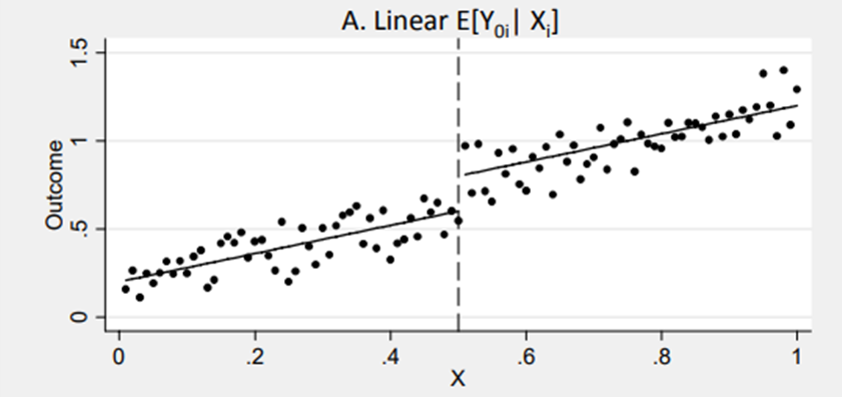
\includegraphics[width=0.6\textwidth]{./IMG/RDD1.png} 
    \caption*{RDD: treatment effect visualization example,\\ linear, common slope.}
    \label{fig:my_label}
\end{figure}    
  
    
\end{frame}
%---------------------------------
\begin{frame}{Regression discontinuity design -- potential problems}
\begin{itemize}
    \item[I.a] Misspecification of the model/functional form, which is used to estimate treatment effect.\\
    \bigskip
    Linearity is often the default approach (assumption) in regression models. However, this may not reflect real DGP. For proper treatment effect estimation, model should be accurately formulated. If appropriate, use quadratic forms, higher polynomials or LOESS (locally estimated scatterplot smoothing).
\end{itemize}
\begin{figure}
    \centering
    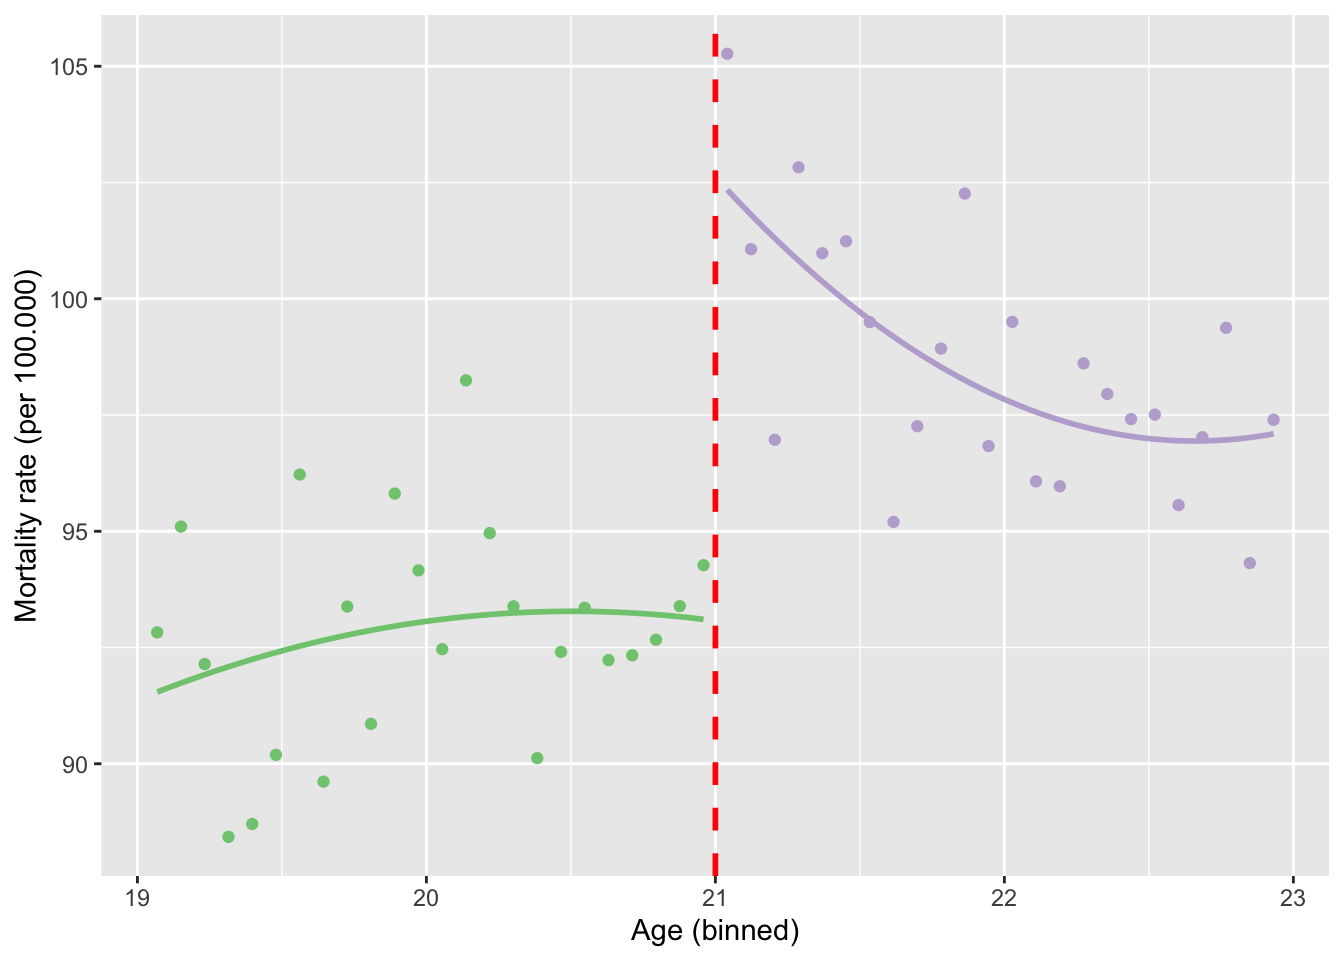
\includegraphics[width=0.55\textwidth]{./IMG/RDD2.png} 
    \caption*{True outcome function can be non-linear.} \label{fig:my_label1}
\end{figure}    
\end{frame}
%---------------------------------
\begin{frame}{Regression discontinuity design -- potential problems}
\begin{itemize}
    \item[I.b] Misspecification of the model/functional form, which is used to estimate treatment effect.\\ 
    \bigskip
    Possibly, once a nonlinear relationship is modelled correctly, discontinuity disappears as it was caused by a misspecification in the functional form. In the plot below, the correct relationship is specified by a curve. If we use a linear relationship, we might observe a (spurious) discontinuity.
\end{itemize}
\begin{figure}
    \centering
    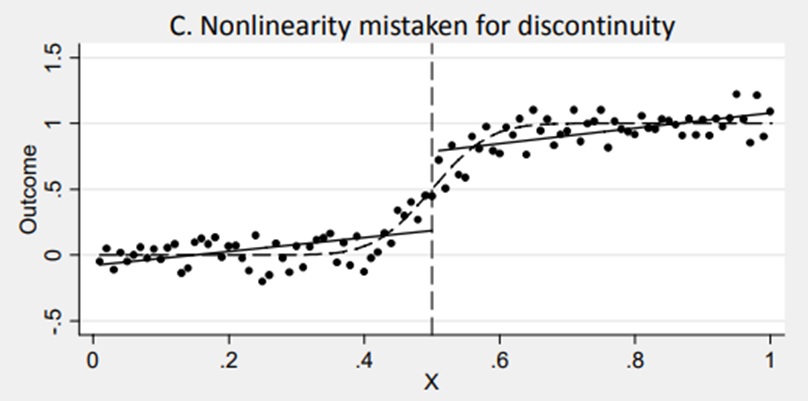
\includegraphics[width=0.55\textwidth]{./IMG/RDD3.png}
    \caption*{``Discontinuity'' caused by functional misspecification.} \label{fig:my_label2}
\end{figure}    
\end{frame}
%---------------------------------
\begin{frame}{Regression discontinuity design -- potential problems}
\begin{itemize}
    \item[II.] Diffusion of the treatment.\\ \bigskip \small
    
    RDD assumes that all individuals below (or above) the cutoff point received the treatment and vice versa.\\ \smallskip
    In reality, the treatment and the control groups can be ``contaminated''. Say, despite mandatory attendance policy (below a given grade average), some students do not attend classes. Alternatively, individuals below (or above) the cutoff might be \textit{allowed} to attend special classes or programs. \\ \medskip

    \textbf{RDD fuzzy design}: cut off is probabilistic. Methodology \& solutions:\\

    \begin{itemize}
        \item Acknowledge possible issues, but still run RDD model comparing eligible vs ineligible individuals.
        \item Use eligibility as an instrument (IV). First estimate treatment probability, then use RDD to estimate the treatment on the treated.
        \item \textcolor{blue}{\underline{\href{https://onlinelibrary.wiley.com/doi/10.1111/1468-2354.t01-1-00055}{Methodology details provided by: van der Klaauw, 2003}}}
    \end{itemize}


\end{itemize}
\end{frame}
%---------------------------------

\subsection{Propensity score matching}
\begin{frame}{Propensity score matching}
    Greene 19.6.2
\end{frame}
%---------------------------------





%---------------------------------
\begin{frame}{Treatment effects - additional literature}
\textbf{Treatment effects}\\
\medskip
For detailed \& technical discussion, see:\\
\medskip
\begin{itemize}
\item[1.] Greene: Econometric analysis, chapter 19.6
\medskip
\item[2.] Angrist, Pischke: Mostly Harmless Econometrics
\medskip
\item[3.] Cameron, Trivendi: Microeconometrics, Methods and Applications, chapter 25
\medskip
\item[4.] Wooldridge: Econometric analysis of C-S and panel data, chapter 21 Estimating Average Treatment Effects
\end{itemize}
\end{frame}
%---------------------------------
%---------------------------------------------------------------------
\end{document}